
\section{Introduction}\label{ctmixtures:sec:introduction}

The emerging field of cultural evolution is the study of cultural change in humans and other animals as a Darwinian evolutionary process, and encompasses research in biology and the social sciences.  As part of an ``extended synthesis’’ \citep{Pigliucci2010}, cultural evolution extends  the notion of ``descent with modification’’ to include the learning and accumulation of cultural information between generations, and explicit study of the differences in structure and pattern between genetic and cultural transmission.  Beginning with the seminal work by Cavalli-Sforza and Feldman 
\citeyearpar{CF1981} and later by Boyd and Richerson \citeyearpar{BR1985}, the study of these differences has focused a great deal of attention on cognitive and psychological biases that create population structure.  Over the past thirty years experiments, observational studies, and theoretical models have come together to create a picture of human social learning which is biased towards conformity under many circumstances and the observation of success, positive payoffs, and social prestige as a basis for selecting those from whom one learns or imitates \citeeg{richerson2005not}.  

Most of the evidence for this emerging picture of human social learning comes from controlled experiments and observational studies of living populations.  Most of it is conducted by psychologists and anthropologists \citep{whiten2016cultural,mesoudi2016evolution}.  Archaeologists and paleoanthropologists seeking to study the evolutionary history of social learning are consumers of this body of theory.  There is nothing wrong with being a consumer of evolutionary theory---every discipline involved in applying Darwinian insights to human social behavior is a consumer in some area---but we must also be producers of methods needed apply that theory to the unique empirical phenomena we study.  Our job consists, at a high level, of building methods for constructing models appropriate to the kinds of data we possess, understanding how to best to assess the fit between those models and our data, and finally, understanding the limits of our ability to do so given the nature of the empirical phenomena we study.  

This paper addresses the limits of our ability to select among detailed, individual-level models of cultural transmission in most archaeological situations.  Initial optimism applying mathematical models of cultural transmission to archaeological data \citeeg{Neiman1995,eerkens2005cultural,Lipo1997,Shennan2001ceramic,Jordan2003} has given way to a more nuanced view of our ability to discriminate between models \citep{barrett2019equifinality,premo2010equifinality,kandler2019analysing}.  A growing body of work is aimed at assessing the causes of equifinality between cultural transmission models given archaeological data, for example assessing the effects of time averaging \citep{Madsen2012,Porvcic2014,Premo2014,perreault2018time} and non-stationary population sizes \citep{Rorabaugh2014,kandler2018generative}.  The hope is that methodological development will help us understand, and correct for, these sources of equifinality so that we can proceed with ``model selection'' and fitting (albeit in a more sophisticated way) and still work with the kinds of transmission models that other anthropologists and social psychologists employ (especially those derived from Boyd and Richerson's seminal work on ``dual inheritance theory'').  

There is no question that we can empirically detect different types of social learning modalities in controlled experiments \citep{kempe2014experimental,mesoudi2006bias,whiten2016cultural,mesoudi2008cultural,Mesoudi2008a,Mesoudi2014}.  Experiments and detailed observational studies of living populations generate fine-grained data about who individuals learn from and what covariates affect ``chains'' of transmission.  Archaeologists, even in the best of circumstances, always face data which is coarse-grained compared to  that available in experimental settings.  To one degree or another, the data we generate from archaeological deposits are estimates of some population-level prevalence of cultural traits.  

Understanding the limitations of using coarse grained data to perform model selection is crucial for archaeology and paleoanthropology,   The main approach to identifying the best fit cultural transmission model for a data set has been to construct univariate statistical tests or distributional expectations for various summary statistics.  Examples of summary statistics employed in this model fitting approach include richness or diversity (evenness) measures, the average amount of time traits survive in a population, their turnover properties, or the degree to which frequency data match distributions known to arise in various “null” models \citep{Shennan2001ceramic,shennan2008style,Bentley2003,shennan2008style,Kandler2013,Kandler20150905}.  These statistics are highly attractive for archaeological purposes because most are easy to calculate from standard descriptions of archaeological assemblages without additional measurements on individual artifacts and thus allow the study of previously described data sets.  

This approach has now been employed in enough studies, and with enough replications on the now-paradigmatic ceramic data from the European Neolithic Merzbach Valley, that we can evaluate its performance.  Kandler \citeyearpar{Kandler20150905} notes that after five separate analyses of the Merzbach data using a variety of summary statistics and approaches, the results remain in conflict.  It is not clear whether the data are consistent with a hypothesis of neutrality, or anti-conformity/novelty seeking, or whether both are reflected in different assemblages.  

There has been much less focus on the crucial question of whether some of the equifinality we face is simply structural.  By ``structural'' equifinality, I mean that the models we expect to be able to identify cannot be distinguished because they overlap too strongly in their outcomes, with any possible data we can obtain.  This paper is an attempt to outline a major cause of structural equifinality in cultural transmission modeling:  the inherent variability of social learning modes within real populations.  The simulation experiments reported here seek to understand whether individual variability in cultural transmission and social learning strategies renders our models impossible to distinguish given coarse grained data, and what effects that sampling and time averaging have on our ability to distinguish the true data generating process behind our data.

This study employs simulation from several data generating models, and employ multiple summary statistics and a powerful machine learning classifier capable of finding highly nonlinear decision boundaries to determine whether it is even possible to discriminate between our theoretical models.  If we can, then it is reasonable to expect that further methodological research on ways to ``correct'' or avoid sources of equifinality may be fruitful.  If we cannot distinguish between models, even in the idealized case, then I believe we must question the utility of attempting to perform the kind of microevolutionary model fitting that many of us have been attempting with archaeological data.  

The results indicate that populations with mixtures of bias can be distinguished from a reference population of unbiased copiers very accurately given a full population census and the absence of time averaging.  In this sense, equifinality between these theoretical models may not be structural even with coarse-grained data.  However, the introduction of sparse sampling and the interaction of sampling with time averaging markedly degrades our ability to accurately classify samples as to their model of origin.  Furthermore, the pattern of errors is not symmetric.  With sampled, time averaged data, we are extremely likely to conclude that samples represent various kinds of transmission bias, even when this is not the case.  

This result deepens the skepticism we should feel as archaeologists about the ability to apply detailed social psychological models to most archaeological data.   Instead of attempting to adapt our data so that we can apply microevolutionary models, we may be better off adapting our models to the data and empirical record we actually possess.  This means looking at coarser grained models and coarser grained research questions which may better match the unique strengths of a diachronic, aggregated record of human evolution.  

\section{Within Population Variation in Social Learning:  A Cause of Structural Equifinality?}\label{ctmixtures:sec:structural-equifinality}

The microevolutionary models of cultural transmission we typically employ in archaeology draw structurally upon the mathematical core of classical population genetics, but add inheritance structures and social learning modes informed by observations across the social sciences \citep{CF1981,BR1985}.  The core models in dual inheritance theory richly vary in the cognitive biases they describe, but all still tend to ignore significant sources of population structure or variation.  All tend to assume \emph{panmixia} as a simplifying assumption, and most tend to depict the population-level consequences of sets of individuals who employ a single learning mode or class of cultural ``parent'' to learn from \citep{wimsatt2019articulating}.   

Real populations, as opposed to those depicted in much of our modeling, have rich structure.  Human populations are mixtures of people of different ages, genders, and propensities for individual versus social learning.  There also appears to be variation among populations and major cultural lineages in these mixtures of social learning traits.  Detailed experimental and observational studies are just beginning to document this variation \citep{whiten2016cultural,yaveroglu2002cultural,tweed2002learning,chang2011cultural,enquist2007critical,csibra2009natural,tomasello2016ontogeny,lopez2010attention,berl2015cultural,mesoudi2015higher,mesoudi2016evolution}  People can vary in these propensities over the course of their lifetimes \citep{lehmann2013optimal,demps2012social,correa2009children,mesoudi2016evolution}, making demographic factors important in modeling the population-level effects of individual social learning processes.    

Even if different ways of learning from parents and peers are distinguishable from individual level data, we should not automatically assume that their population level consequences are distinguishable, when there is variation in the population.  Processes which are distinguishable with transmission chains, for example, may have opposing effects on population-level summary statistics.  A population comprised of conformists who prefer to learn and stick with the ways that have worked in the past would tend to display fewer variants in the population than expected in a neutral equilibrium, and more concentration of frequency on a small number of traits.  A population comprised of those who prize novelty and exploration of ``new'' traits will tend to display more variants than expected, with more evenness among trait frequencies.  A real population that combines individuals with both propensities 
would display a mixture of these population-level consequences.  In other words, some of the effects easily visible at the individual level may ``cancel out''.  If that is the case, can we distinguish a mixture of these social learning biases, from a population of unbiased copiers?  

\begin{figure}[ht!]
  \centering
  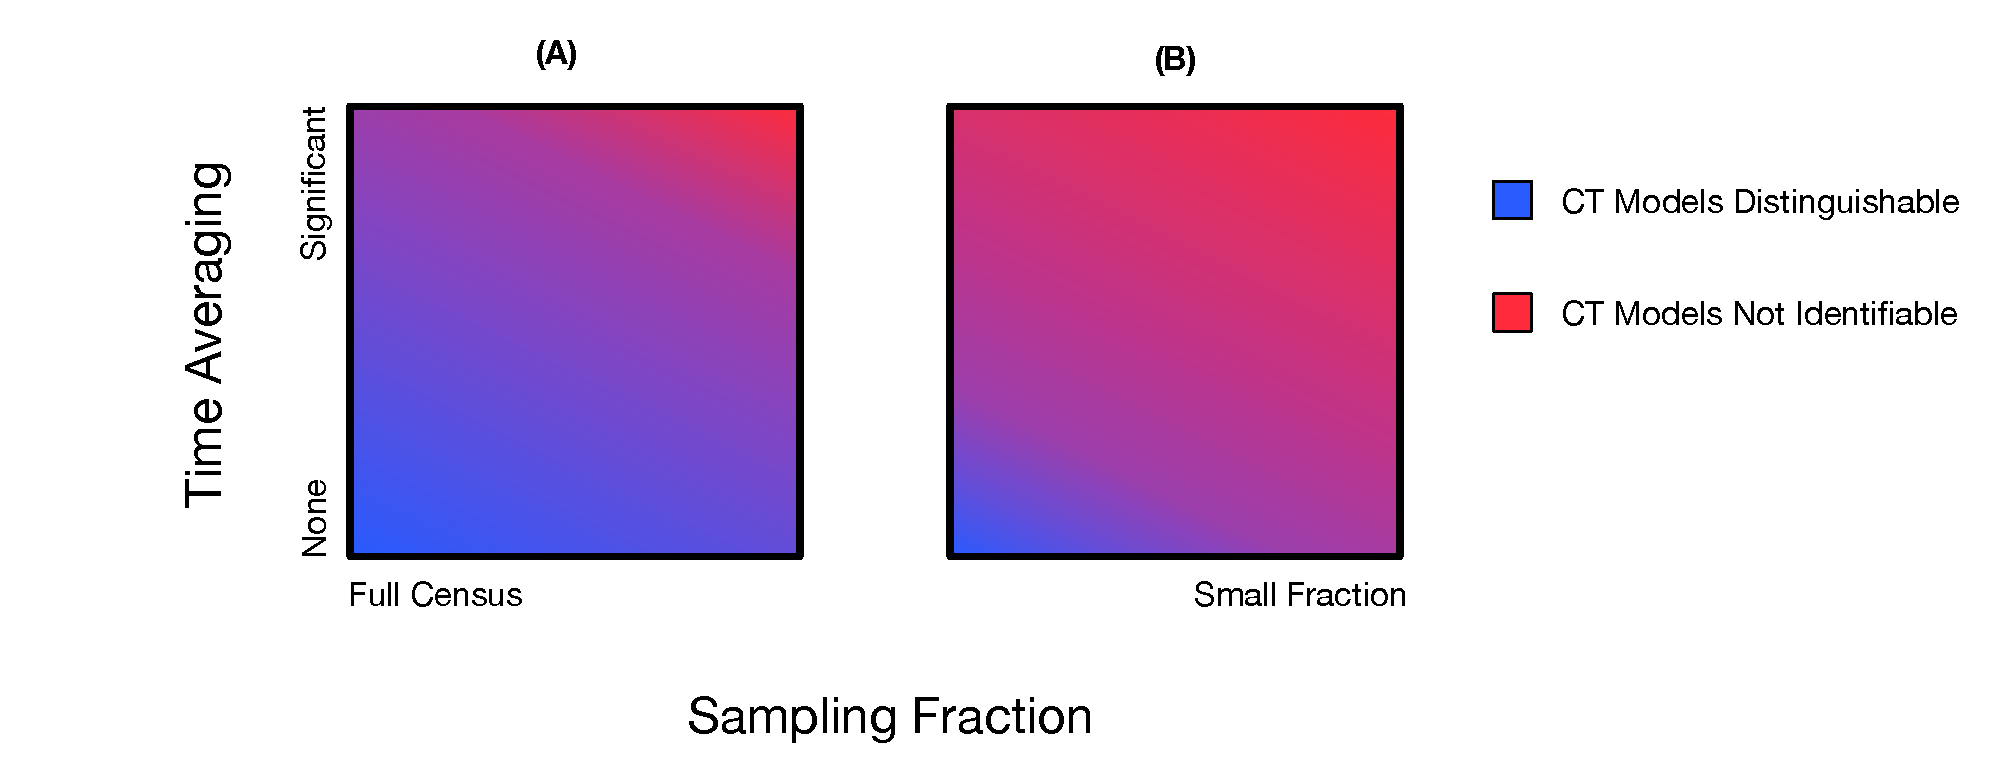
\includegraphics[scale=0.5]{graphics/ctmixtures/equifinality-transmission-bias-scenarios.pdf}
  \caption{Two scenarios for how equifinality may affect our ability to empirically distinguish between different models of cultural transmission given the effects of sampling and time averaging.}
  \label{ctmixtures:fig:equifinality-scenarios}
  \end{figure}

This question becomes even more concerning when we combine the “structural” possibility of equifinality just described with the “methodological” sources of equifinality previously discussed:  sampling and the time averaging characteristic of aggregated, time transgressive data.  This question is depicted schematically in Figure \ref{ctmixtures:fig:equifinality-scenarios}.  In the left panel, under mild to moderate amounts of time averaging and with reasonable sample fractions, our ability to discriminate between models may be relatively strong, with equifinality restricted to situations with small sample size and in assemblages with significant duration.  The right hand panel depicts the other end of a continuum of possibilities:  our ability to identify transmission models given data might be quite rare across a range of values relevant to archaeological inquiry.  This paper is an attempt to determine where we might stand between these two poles.  Given even simplified models of mixed social learning processes, can we tell apart their population level consequences, especially with limited samples and in the presence of time averaging?

\section{Methods}\label{ctmixtures:sec:methods}

\subsection{Study Design}\label{ctmixtures:sec:study-design}

I approach this question by simulating populations with mixtures of social learning or transmission biases.  In particular, I examine populations comprised of mixtures of conformist and anti-conformist individuals, along with a ``reference'' population of unbiased copiers \citep{BR1985}.  The simulated populations are censused at sampling intervals and trait counts recorded.  This allows us to later perform a variety of ``data collection regimes'' which simulate the effects of archaeological sampling and the time averaging effects of aggregate deposition in the archaeological record.  It also allows analysis at the single trait level, or the composition of traits into ``classes'' which simulate the effects of archaeological classification, since most efforts to fit cultural transmission models to real data have accepted existing classification schemes as input to the model fitting.  

The output of the simulation runs are simulated archaeological observations of trait or class frequency count at a variety of levels of sample size and time averaging ``treatments'' from the same underlying data generating processes.  This allows us to examine our ability to distinguish between data generating processes depending upon the ``treatment'' levels, given a method for predicting which data generating process produced the data points observed.  In the next section, I describe a predictive modeling approach, adopted from machine learning, for measuring equifinality as error in properly predicting the known data generating process for our simulated data.  

\subsection{Measuring Equifinality Through Classification Error}
\label{sec:equifinality-classification-error}

The common models of cultural transmission employed by archaeologists are stochastic in nature, and thus when we take samples from simulations of those models, we will observe a distribution of results for any summary statistic we choose to observe.   To the degree that several models generate separable distributions for the chosen summary statistics, we will be able to infer the most probable data generating model given values of those statistics.  If the distributions of summary statistics have some overlap, the level of certainty with which we can predict the correct data generating model will decline overall, and perhaps be no better than chance in the region of overlap.  

This generic situation is shown schematically in Fig.
\ref{ctmixtures:fig:distributional-scenarios}. Here, three pairs of probability models
are represented by 500 measurements each of two continuous predictors variables (e.g., a diversity index).
In the left panel, the pair of models do not overlap in their outcomes.
Given a data point, we can assign it to Model 1 or Model 2 with
virtually no error, and thus we would consider models 1 and 2 to be
distinct and not equifinal at all. The situation in the middle and right
panels of Figure \ref{ctmixtures:fig:distributional-scenarios} is different. There is
some overlap in the middle panel, and very strong overlap in the right
panel. In the right hand panel, in fact, there is enough overlap that on
average, our ability to assign a randomly chosen data point to the
correct model is no better than chance. Intuitively, we would say that
there is some equifinality in the middle panel, and that the two models
in the right hand panel were strongly equifinal.

\begin{figure}[ht]
\centering
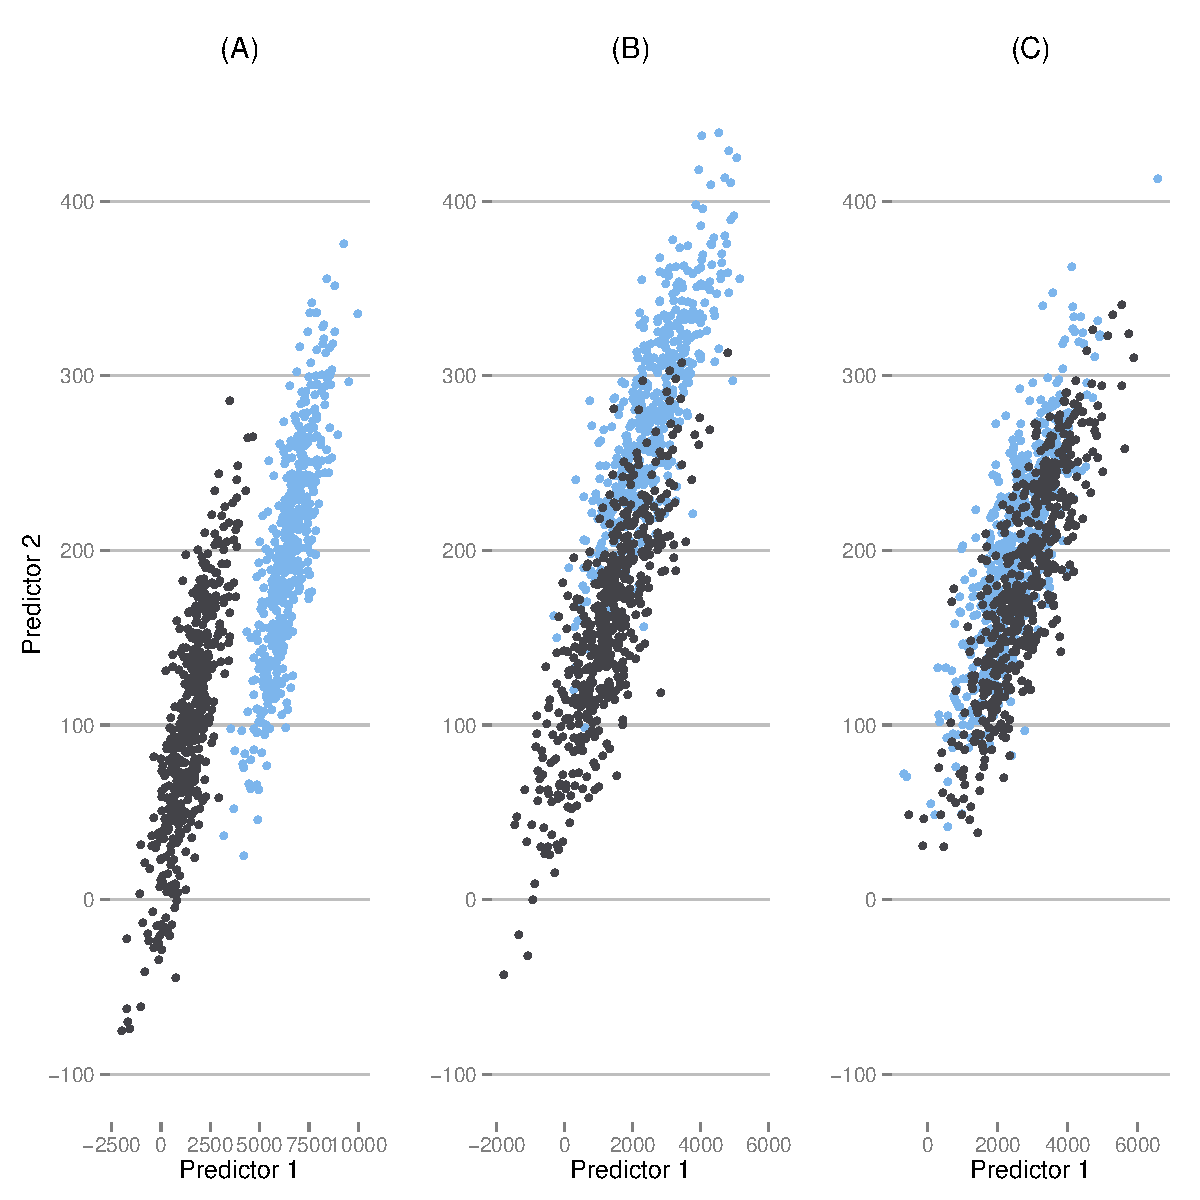
\includegraphics[scale=0.6]{graphics/ctmixtures/distributional-overlap.pdf}
\caption{Simple example of model outcomes with different degrees of distinguishability given two summary statistics: (A) simulated data points from two fully separate models, (B) two models with a limited overlap region, (C) and two models whose outcomes are highly overlapping.}
\label{ctmixtures:fig:distributional-scenarios}
\end{figure}

Measuring the overlap between the measured outcomes of theoretical models thus provides a way to determine their inherent or structural equifinality given a set of observable summary statistics or observational variables.  When theoretical models are simple enough to have solvable equations, it may be possible to perform an analysis of distributional overlap using mathemetical tools such as the Kullback-Leibler divergence between their resulting probability distributions \citep{burnham2002model}.  In the kind of cases discussed in this paper, with mixtures of social learning modes in a single simulated population, we need a numerical and thus statistical approach.  We will operationalize measurement of distributional overlap by producing samples from each theoretical model, calculating or other producing the observable variables or summary statistics, applying any simulated data collection treatments (such as specific sampling regimes), and then attempting to ``predict'' which data generating model generated each data point.  The error rate in predicting the correct model is a quantitative measure of \emph{how much equifinality} there is between models, given a set of predictor variables and data collection treatments.  

In more formal terms, we define measurement of equifinality as the error in performing a classification task, in the machine learning sense \citep{murphy2012machine}.  Given a set
of models \(\mathcal{M}_1 \ldots \mathcal{M}_n\), we can measure
equifinality as the minimum possible error achievable in correctly
assigning simulated data points to the data generating model which produced them,
given measurement of a set of predictor variables or ``summary statistics.'' In the classification task, we ask which model has the highest probability for
a given data point, given the conditional density of the data and
models. This sounds exactly like Bayes' theorem, and in fact we can
write the classification problem as follows, where
\(Y \in 1, \ldots, K\) refers to each of \(k\) models, and
\(X_1, \ldots, X_p\) refer to \(p\) different predictor variables.

\begin{equation}
\mathbb{P}(Y | X_1, \ldots, X_p) = \frac{\mathbb{P}(Y_i) \mathbb{P}(X_1, \ldots, X_p | Y)}{\mathbb{P}(X_1, \ldots, X_p)}
\label{eq:bayes-rule-classification}
\end{equation}

\(\mathbb{P}(Y)\) plays the role of the prior distribution, and reflects how prevalent we expect each label or model to be in the population.  In a true empirical study this might be uniform---if we had no reason to suspect that a model may be more likely than another \emph{a priori}, or we may have substantive reasons for weighting models.  For example, models may capture the prevalence of a genetic factor, and we may have quantitative evidence for that prevalence.  In a theoretical study such as this one, we are simulating equal numbers of samples from each theoretical model, and thus the term will be constant and cancel out.  The data points in a classification problem are given, and
thus the denominator is also a constant. The most probable class for a given
data point reduces, therefore, to the mode of the likelihood function:

\begin{equation}
Y_{pred} = \argmax_y \mathbb{P}(X_1, \ldots, X_p | Y)
\label{eq:map-class-bayes}
\end{equation}

This is the \emph{Bayes classifier} for a controlled simulation
experiment, and its error rate in separating data points by model is
called the \emph{Bayes error}. This is the lowest possible error in
separating the models given the data
\citep{devijver1982pattern, fukunaga1990introduction, hastie2009elements}.
The Bayes error is zero when we can correctly identify each data point
as to its model of origin (as in the left panel of Fig. \ref{ctmixtures:fig:distributional-scenarios}, and rises as two models overlap in the
measurement space. With sufficient overlap, the Bayes error could
approach 0.5, which represents a prediction rule which is no better than
chance, or conceivably rise even further, indicating that our classifier performs even worse than coin-flipping.\footnote{Error rates can obviously be higher than 50\% in an empirical study, but in a controlled simulation study like the present paper, error higher than a coin-flip is indicative of a problem with the experimental setup.}

Unfortunately, we can almost never directly calculate the Bayes error
rate for a prediction or classification rule, because we rarely have an
expression for the likelihood function of our transmission models in the
spaced formed by the predictor variables. Bayes error can be directly calculated, in fact, only for
a small number of cases, such as Gaussian distributions with a shared
covariance
matrix.  There is a large literature, especially in pattern recognition and language classification, on approximating upper bounds for the Bayes error of a classifier, because it is highly useful to know when you cannot improve a recognition system or classifier any further \citep{Antos:1999dn, Dobbin:2009du, McLachlan:1975eo}.  Most such upper bounds are based upon parametric models, and use estimates of a distance metric between the classes being distinguished (typically, the Mahalanobis or Bhattacharyya distance) \citep{devijver1982pattern}.  Such bounds are difficult to apply in situations where we have complex social learning models, whose probability density functions in the space of measured variables are typically unknown.  

Despite the fact that we can rarely calculate the Bayes error rate, it
is useful as an operational definition for equifinality, since it
measures our uncertainty about model choice given a set of measurable
variables. In practice, we approximate the Bayes error by employing classifier algorithms which are able represent complex relationships between all of the predictor variables in order to get as close to the Bayes error rate as possible.  This generally means using methods with higher model ``capacity'' than the linear models familiar to most archaeologists (such as logistic regression or linear discriminant analysis).  Formally we seek methods with high Vapnik-Chervonenkis (or VC) dimension, which measures the ability to represent complex decision boundaries between classes \citep{vapnik2013nature}.  At present, methods such as boosting, bagging, and ensemble approaches that combine weaker methods such as decision trees with boosting combine high capacity with very low error across many benchmark cases \citep{hastie2009elements}, and thus come closest to estimating the
Bayes rate \citep{tumer2003bayes}.  

\subsection{Simulation Modeling of Cultural Transmission Mixtures}\label{ctmixtures:sec:ct-mixture-modeling}

In order to measure the overlap between various theoretical mixtures of social learning strategies, I built simulation models for the scenarios given in Table \ref{ctmixtures:tab:models}.  The outcomes of all four transmission models are derived by simulating the
dynamics of the model in an agent-based framework that allows each agent to be assigned a different transmission rule.  All simulations employ
the Moran dynamics, where one individual engages in a copying event at
each elemental step
\citep{moran1962statistical, moran1958random, aoki2011rates}.
Innovations are modeled using the ``infinite alleles'' approximation,
where every innovation is new to the population \citep{Ewens2004}.
Simulations were performed using the CTMixtures software package,
available as open source
software.\footnote{\url{https://github.com/mmadsen/ctmixtures}} The
parameters for all simulation runs are given in Table
\ref{tab:parameters}. Where there is a range given (e.g., innovation
rate), the parameter is treated as a prior distribution and each
simulation run is assigned a uniform random value from the range. This
ensures good coverage of the parameter space given 25,000 replicates for
each of the 4
models.\footnote{The use of a good prior distribution for parameter ranges also results in simulation data that are usable for later data fitting by approximate Bayesian inference \citep{Beaumont2010, Crema2014, Csillery:2010jd, Marin2012}.}

\begin{table}[ht]
    \begin{tabular}{ll}
        \hline
        Model Code & Model Description \\ 
        \hline
        Unbiased & Population with only unbiased copiers \\
        Equal Mixture & Equal numbers of conformists and anti-conformists \\
        Conformist Dom & 70\% conformists with 30\% anti-conformists  \\
        AntiConf Dom & 70\% anti-conformists with 30\% conformists \\
        \hline
    \end{tabular}
    \caption{Theoretical models that were simulated as part of this study.}
    \label{ctmixtures:tab:models}
\end{table}



\begin{table}[htb]
\begin{tabular}{lc}
\hline
Parameter & Value or Interval \\ 
\hline
Innovation rate (in $\theta$ scaled units)  & $[0.1, 5.0]$   \\
Probability of conformism & $[0.05, 0.25]$ \\
Probability of anti-conformism & $[0.05, 0.25]$ \\
Sample fractions & 0.1 and 0.2 \\
Time averaging intervals (units of 100 individuals) & 10, 20, 50, 100 \\
Population size & 100 \\
Number of trait dimensions (loci) & 4 \\
Initial traits per dimension & 10 \\
\hline
\end{tabular}

\caption{Parameters for simulation runs across the four models studied.  Intervals are treated as prior distributions, and each simulation run is assigned values derived from a uniform random sample on the interval indicated.  Lists of values are all applied to every simulation run (e.g., there is both a 10\% and a 20\% sample from each simulation run.  Single values are applied to every simulation run, and represent a point prior.)}
\label{tab:parameters}
\end{table}

Simulated populations are 100 individuals in size, because most
archaeological studies of cultural transmission have focused upon
situations where population sizes are assumed to be small. 
Each simulated individual carries 4 different
traits at any time, which are treated as separate loci or dimensions.  Trait frequencies are tracked on a per-locus basis, and combinations of loci are tracked in order to simulate archaeological ``types'' or classes which include multiple dimensions of variation.

Regardless of transmission model, social learning involves no interaction effects between loci in this study. The
population is seeded with 10 randomly chosen traits at each locus as a
starting configuration. The evolution of each simulated population proceeds
for 4 million elemental steps, which is equivalent to about 40,000
copying events on average per individual. This value was chosen by
performing simulations at 1 million time step intervals and verifying
that the distribution of a key statistic (the number of traits per Loci)
had stabilized. This occurred in most cases between 2 and 3 million
steps, and in all cases between 3 and 4 million, so the last value
was chosen.\footnote{The analysis underpinning this decision is available in the Github repository at \url{https://github.com/mmadsen/experiment-ctmixtures/analysis/verification}.}
At the end of 4 million simulation steps, a suite of variables are
measured from each of the 25,000 replicates and stored for analysis.


\subsection{Summary Statistic Selection}\label{ctmixtures:sec:variable-selection}

Since most previous work on identifying transmission mode from archaeological data employ single diagnostic variables, and begin to display equifinality under realistic data collection conditions, it is reasonable to examine whether using multiple variables will yield more discriminatory power in the same contexts.  By representing the outcomes of transmission models in a higher dimensional space, it should be easier to find a decision boundary (``separating hyperplane'') that correctly predicts the model which generated each data point, if such a boundary exists.  

\begin{table}[ht]
\begin{tabular}{ll}
\hline
Variable                                    & Model Variable \\ 
\hline
Cross-Tabulated Class Richness  (Class)         &  num\_trait\_configurations      \\
Slatkin Exact (Class)           & configuration\_slatkin       \\
Shannon Entropy (Class)  &  config\_entropy \\
IQV Diversity (Class)  & config\_iqv \\
Neiman $T_f$ (Class) & config\_neiman\_tf \\
Slatkin Exact (Max for Locus)                    & slatkin\_locus\_max       \\
Slatkin Exact (Min for Locus)                     & slatkin\_locus\_min      \\
Slatkin Exact (Mean for Locus)                   & slatkin\_locus\_mean       \\
Shannon Entropy of Trait Frequencies (Min)      & entropy\_locus\_max       \\
Shannon Entropy of Trait Frequencies (Max)       & entropy\_locus\_min      \\
Shannon Entropy of Trait Frequencies (Mean)      & entropy\_locus\_mean      \\
IQV Diversity Index (Min)     & iqv\_locus\_max \\
IQV Diversity Index (Max)     & iqv\_locus\_min \\
IQV Diversity Index (Mean)    & iqv\_locus\_mean \\
Trait Richness (Min)   & richness\_locus\_max \\ 
Trait Richness (Max)   & richness\_locus\_min \\
Trait Richness (Mean)    & richness\_locus\_mean \\
Kandler-Shennan Trait Survival (Min)   & kandler\_locus\_max \\
Kandler-Shennan Trait Survival (Max)   & kandler\_locus\_min \\
Kandler-Shennan Trait Survival (Mean)   & kandler\_locus\_mean \\
Neiman $T_f$ (Min)   & neiman\_tf\_locus\_max \\
Neiman $T_f$ (Max)   & neiman\_tf\_locus\_min \\
Neiman $T_f$ (Mean)   & neiman\_tf\_locus\_mean \\
\hline

\end{tabular}

\caption{Variables measured from each transmission model simulation sample.  The parenthetical expression records whether the variable was calculated for cross-tabulations of all 4 loci (Class) or represent the order statistics from individual loci (Min/Mean/Max).  The right column records the variable name used within R statistical models, for examining the relative importance of each variable in classifying observations.}
\label{tab:variables}
\end{table}

The predictor variables chosen in this study focus upon measures of richness and
diversity, trait survival over time \citep{Kandler2013}, and the
Slatkin neutrality test \citep{slatkin1996correction, slatkin1994exact}.
Each has been employed in the archaeological literature on identifying
cultural transmission modes, or is a variant on such measures (e.g., IQV
is a normalized version of Shannon entropy), and crucially, all are measurable in standard archaeological contexts using attribute or class frequency data.  This additionally makes most of the variables applicable to the re-analysis of already published data, which is an important usage scenario in archaeological research.   

For the locus-centric variables, each statistic was applied to each
locus separately, and the mean, minimum, and maximum of the values
obtained for each locus were recorded. I collect order statistics
in addition to the mean value, since it is possible that minima and
maxima might be a better discriminator between models than averages. In
addition to the variables calculated upon each of the 4 loci, the traits
at each locus were combined into a cross-tabulation of "classes" which simulates the
process of archaeological classification. Each class represents a
different combination of traits from the 4 loci, and very roughly
simulates observing cultural variation through the lens of a standard
paradigmatic classification \citep{Dunnell1971}. The same variables are
then measured as a function of the class counts.\footnote{The sole exception is the Kandler-Shennan survival time, which is not measured here for the cross-tabulated classes.  Understanding the quantitative behavior of this measure for multidimensional classes of traits is an important open research question, however.} This allows us to
understand whether transmission models are better distinguished on a
per-locus (dimension) basis or by operating on more complex classes that
combine several traits together. The full list of measured variables is
given in Table \ref{tab:variables}.

As a final note on variable selection, in an exploratory analysis for this
project, I tried to include the power law exponent as a summary statistic, given the important work by Bentley and colleagues
\citeyearpar{bentley2004random} and Mesoudi and Lycett
\citeyearpar{Mesoudi2009}.  Proper fitting of power law distributions to empirical data is more difficult than simply determining if a straight line describes the data after double logarithmic transformation; in particular testing if a data set displays a power law is difficult if there are a small number of counts and small sample size \citep{clauset2007power}.  This may be difficult in many archaeological cases where the number of classes may be relatively small (on the order of ten rather than hundreds), and the total sample sizes can be relatively small.  In their study, Mesoudi and Lycett
\citeyearpar{Mesoudi2009} use the cumulative number of adoptions of each
trait over the entire time span of their simulations as the ``frequency''
used to calculate power law
exponents.\footnote{I confirmed this by inspection of the source code for their simulation model, which was provided by Alex Mesoudi.}  This quantity is available in simulation but would unobservable in empirical data.  Whether or not to include power law exponents as predictor variables will depend strongly on the data set in question.  Given the experimental setup used in this study, power law exponents were difficult to calculate in a stable way.  Thus, I did not include them in the remainder of this study, and their discriminatory power in combination with other variables thus remains an open question.

\subsection{Data Collection Treatments}\label{data-collection-treatments}

At the end of each simulation run, after the model has reached a quasi-stable equilibrium (measured as stability in per-locus trait richness), a series of samples are taken from the evolving population.  These samples are taken in ways that correspond to various real-world data collection strategies.  First, a census of the entire population is taken.  This functions as a baseline for the ``most complete'' information we can use to identify transmission modes, and there are also conditions during observational studies or in laboratory experiments where census is possible.  In archaeological studies, anything approximating a census is usually impossible, although Jonathan Scholnick's study of New England gravestones and their makers may approximate this quality of data collection \citep{scholnick2012spatial}.  Second, the simulated population is sampled, at the 10\% and 20\% levels.  Sampled data is ubiquitous in archaeological research, and although the issues involved in mapping artifact samples to their meaning for the underlying population of social learners is complex and unresolved, it is useful to determine whether the overall sample fraction has a measurable effect upon model equifinality.  

Archaeology derives its empirical data by sampling a sedimentary record of artifact discard and trace fossil creation by many individuals, often over large spans of time \citep{schiffer1983toward,Schiffer1987,stein2001review,Stein1987,Stein1993,stein2001review,stein2003big}.  Thus, our data almost never represent synchronic or ``point in time'' samples of the results of human activity \citep{Grayson1998,lyman2003influence,Madsen2012,Porvcic2014,Premo2014}.  Therefore, the simulated samples of cultural transmission in this study are also temporally aggregated over a number of time steps, and the aggregate trait counts used to determine the frequencies of cultural traits over the entire interval.  The population census has no temporal aggregation, and thus does represent a synchronic census.  

Time averaging is implemented according to the schematic in Fig. \ref{ctmixtures:fig:kandler-sampling}.  At the end of the simulation run, sampling begins at a time index calculated to allow time averaged samples to be taken twice, with a gap of 50 ``generations'' to also allow the calculation of the Kandler-Shennan trait survival statistic (although unlike their original study, the values at the start and end times are inherently time averaged in this study, which would be the case in any real archaeological context) \citep{Kandler2013}.

\begin{figure}[p!]
\centering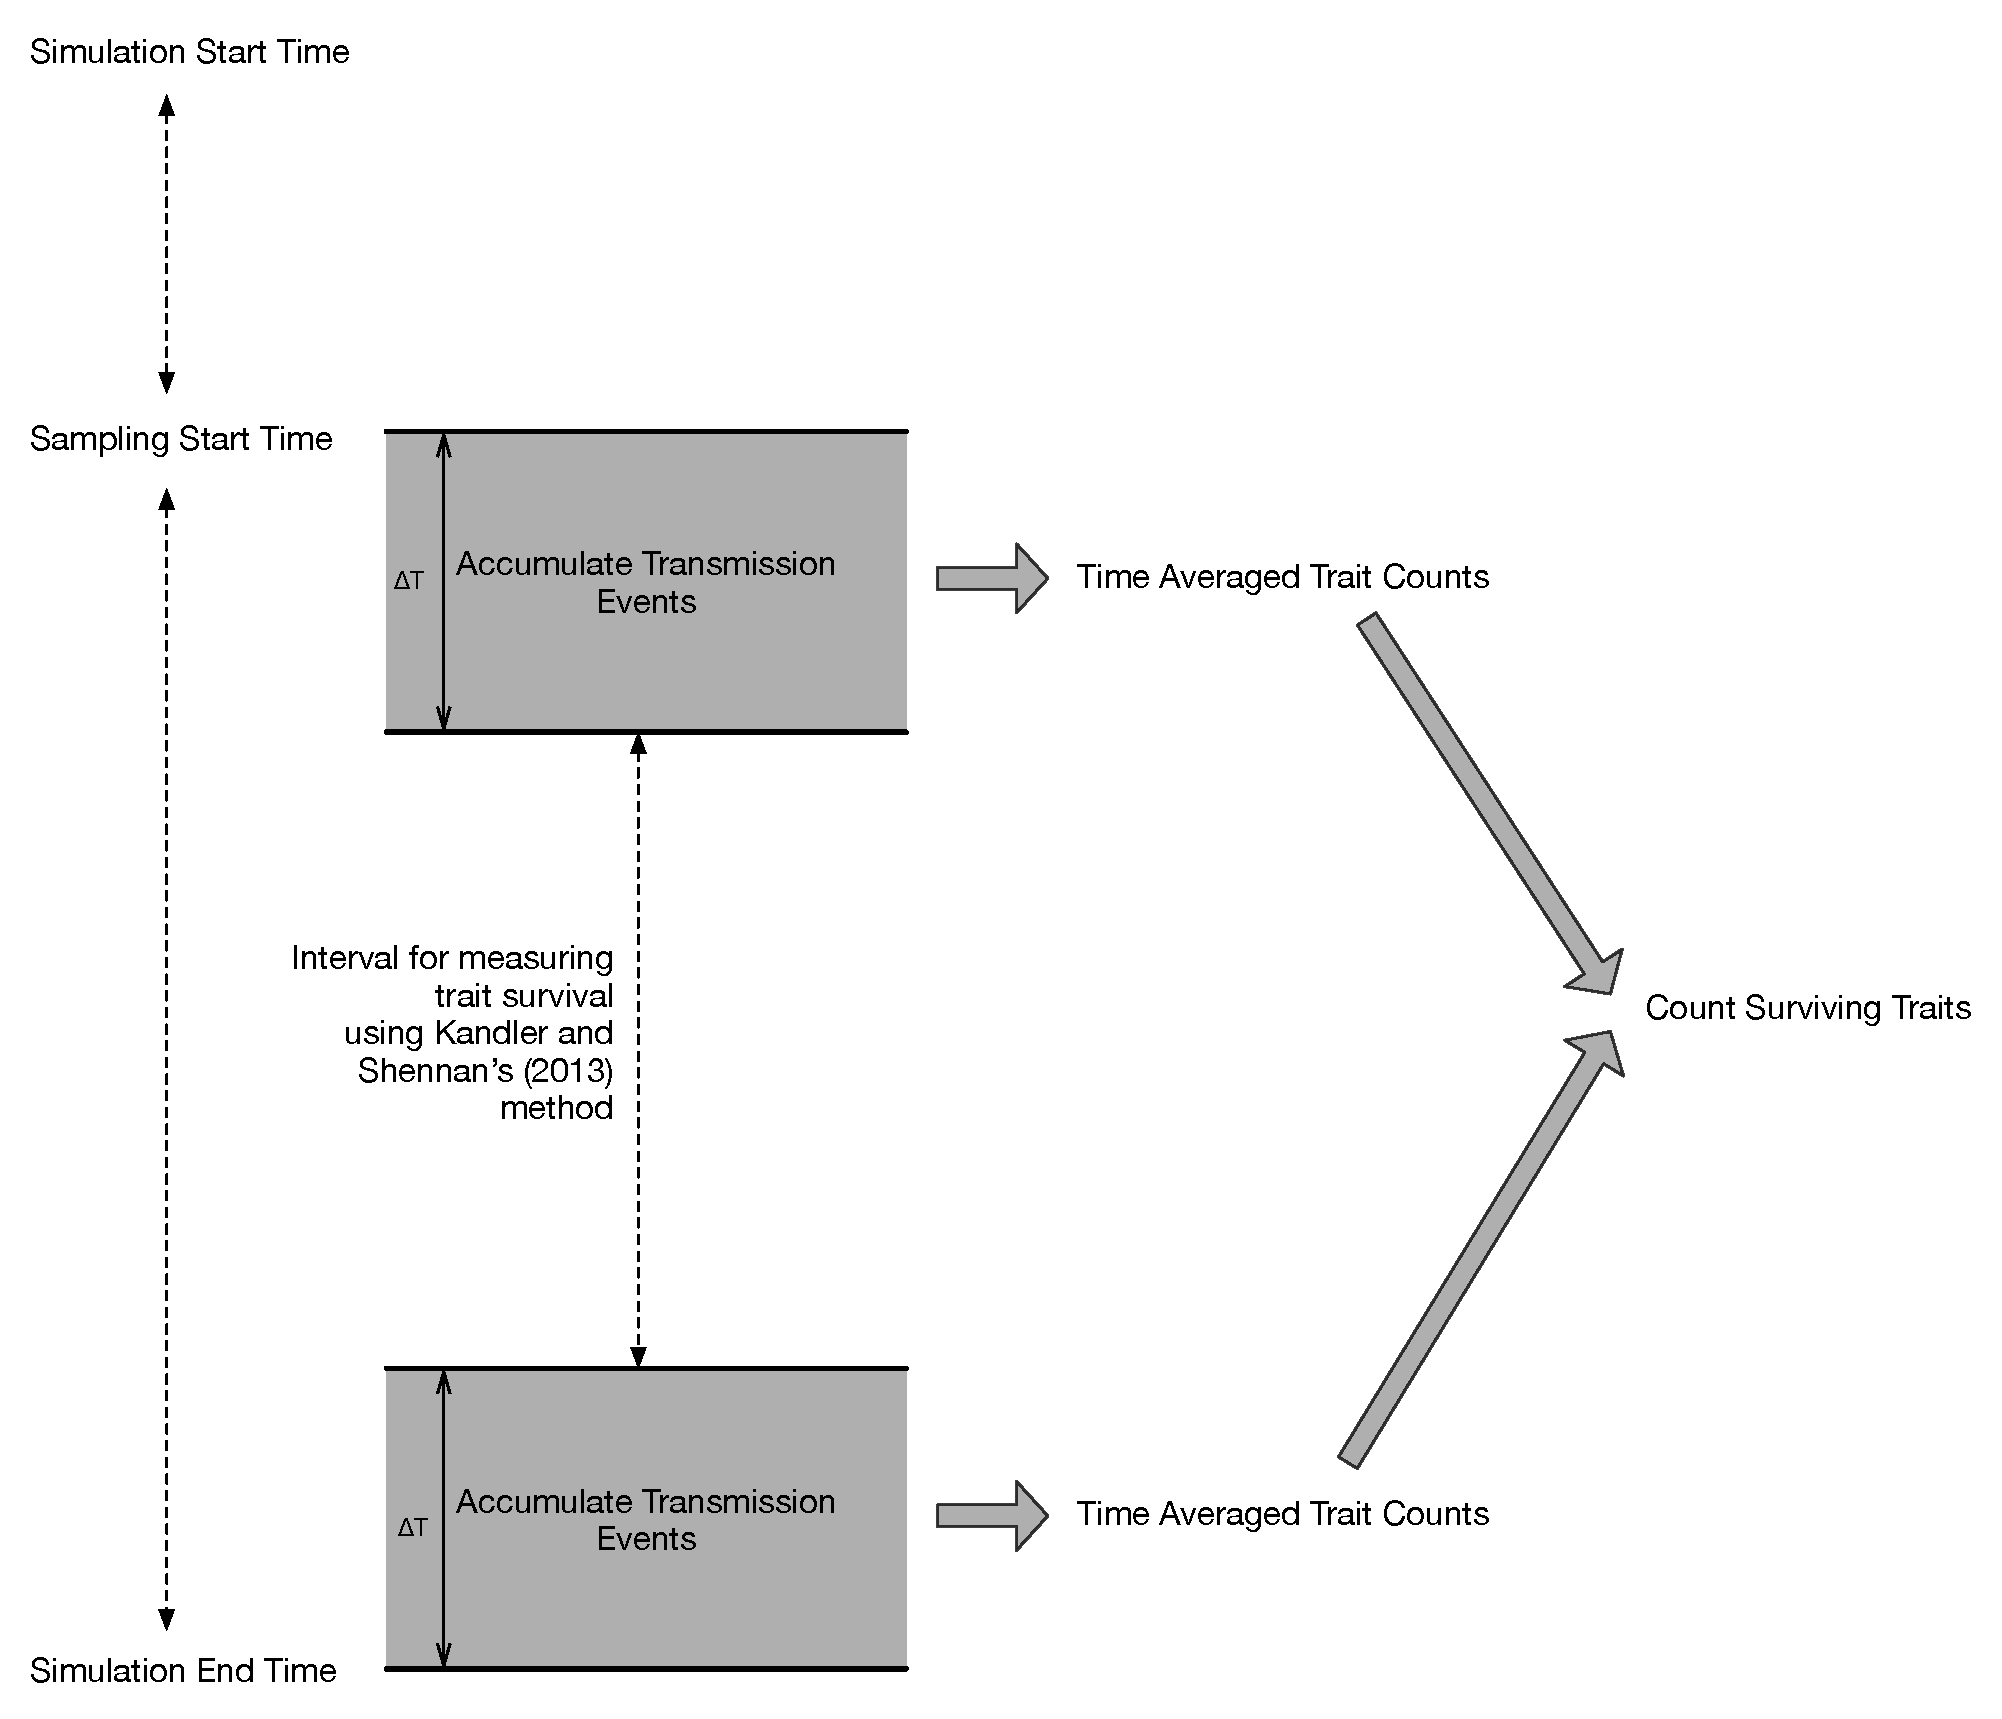
\includegraphics[scale=0.4]{graphics/ctmixtures/time-averaging-with-kandler-sampling.pdf}
\caption{Schematic of how trait survival as described by Kandler and Shennan \citep{Kandler2013} is extended to time averaged samples of transmission events.  Time runs from the start of the simulation run at the top, to the end at the bottom.  The interval of time over which we calculate the Kandler-Shennan trait survival is given as a simulation parameter, and represents the gap in the middle of the diagram.  Before and after that gap are sampling windows during which transmission events are accumulated over some number of simulated ``generations'' (values of 10, 25, 50, and 100 are used in this paper).  Trait survival is then calculated as the number of traits present in the starting time averaged sample of transmission events, which are still present in the ending time averaged sample of events.}
\label{ctmixtures:fig:kandler-sampling}
\end{figure}


\begin{table}[ht]
    \begin{tabular}{ll}
        \hline
        Sampling Strategy & Time Averaging Duration \\ 
        \hline
        Population Census & 0 \\
        10\% Sample & 10 \\
        10\% Sample & 25  \\
        10\% Sample & 50 \\
        10\% Sample & 100 \\
        20\% Sample & 10  \\
        20\% Sample & 25 \\
        20\% Sample & 50 \\
        20\% Sample & 100 \\
        \hline
    \end{tabular}
    \caption{Data collection strategies, applied to every simulation run.  Time averaging duration is given in units of "generations," which are units of 100 time steps (given the population size).  100 generations thus represents 10,000 elemental time steps in the Moran simulation dynamics.}
    \label{ctmixtures:tab:measurement-strategies}
\end{table}

The data collection strategies employed in this study are given in Table \ref{ctmixtures:tab:measurement-strategies}.  Applied to all 23 variables, the study yielded approximately 900,000 samples from the four transmission models listed in Table \ref{ctmixtures:tab:models}.\footnote{All data and analyses for this study are available as part of a Github repository, although large data files are kept on Amazon S3 for long-term storage.  See \url{https://github.com/mmadsen/experiment-ctmixtures} for details.  The published analysis described here is the ``equifinality-4'' data set.}  

\subsection{Classifier Selection and
Training}\label{classifier-selection-and-training}

Classifier algorithms are supervising learning models from statistics
and machine learning that predict a categorical response from a mixture
of discrete or continuous variables \citep{hastie2009elements}. The most
familiar classifiers in archaeological practice are logistic regression
and discriminant function analysis, but neither is competitive with
contemporary ``ensemble'' methods which combine many classifier rules
into a single prediction. In such models, combining predictors can both
reduce the variance of prediction (e.g., bagging added to traditional
classifiers and random forests), and
reduce bias.  Some classifiers, like boosted trees, can do both.

Since the Bayes error rate of comparing two complex transmission models is not something we can calculate or even estimate, we must approximate it using the best performing classifier model available.  A very general result in statistical
decision theory (called, appropriately, the ``No Free Lunch'' theorems)
guarantee that there is no single prediction model that can achieve the
best result with every data set and problem
\citep{wolpert2002supervised, wolpert1997no}. Thus, I took a compromise approach, selecting several algorithms that are known to have excellent performance across a range of data sets, and then performing a pilot study using the four transmission models previously described.  A recent study
compared 179 classifier algorithms on 121 different data sets
(representing the entire UC Irvine Machine Learning Database), and found
that random forests \citep{breiman2001random}, support vector machines,
and gradient boosted classifiers performed the best
\citep{hastie2009elements}. Additionally, some ensemble methods (random
forests and gradient boosted classifiers) provide information on
variable importance as an integral part of the algorithm.  Since understanding which of our 23 variables are useful for separating transmission models is an important aspect of this study, I evaluated random forests against gradient boosted classification trees using small simulated samples from each transmission model.\footnote{The data for this initial comparison are available in the \url{https://github.com/mmadsen/experiment-ctmixtures} repository under the experiment name ``equifinality-2''.}
Gradient boosted models outperformed random forests on these simulated
data, are comparable in computational costs, and are used for all
further results in this paper.

Gradient boosted classification operates by repeatedly fitting a set of
decision trees to the data \citep{AlexeyNatekin2013,hastie2009elements}. In each round, decision trees are fit to the training data, and individual data points scored as errors or successful predictions.  Subsequent trees are fitted by modifying the trees in the direction that minimizes the residual error.  This is equivalent to finding the gradient of the loss function in the space of possible classifier functions, hence the name of the method.  The impact of each gradient step is smoothed by including a ``shrinkage'' factor.  Finally, the gradient steps are ``boosted'' to weight data points by the success in prediction, such that data points that are frequently misclassified become targeted by the algorithm until they can be correctly predicted \citep{freund1995boosting, freund1999short, schapire2012boosting}.  After a specified number of iterations, the class or label membership of each data point is obtained by having each gradient step classifier tree ``vote'' for class membership, and the final answer is the majority vote.  This class of models can also be visualized as repeated refitting of residuals until error is minimized \citep{friedman2001greedy}.  This combination of boosting and iterative function search is very powerful, and gradient boosted models regularly achieve top accuracy in benchmark studies.

In this study, I employ the R package (\textbf{gbm}) for gradient
boosted classification \citep{ridgeway1999state}, with the binomial deviance \(\textrm{log}(1 + \textrm{exp}(-2y\hat{y}))\) as our loss function, where \(y\) is the true
model for a data point, and \(\hat{y}\) is the classifier model's
prediction.  Binomial deviance approximates the ``zero-one'' loss function with one which is differentiable, which is needed for a gradient descent method.  The tuning parameters for this study (number of boosting iterations, depth of classification trees) were selected using 5 rounds of repeated 10-fold cross-validation on the training data \citep{Kim:2009im, kuhn2013applied}.

The full data set of simulation samples, after data collection treatments, was split into two chunks. 80\% of the data were
used to train the classifier model, and 20\% were held back to provide an
unbiased evaluation of classifier performance.  For each comparison of models
reported, the training data were thus fitted 50 times across
different values of the tuning parameters (number of boosting
iterations, and depth of decision trees), and the best performing
parameters chosen from the repeated cross-validation sets. The final model is then constructed using the entire
training set and the optimal parameter values. All classifier tuning,
final model fitting, and test error evaluation was performed using Max
Kuhn's superb \textbf{caret} package for R
\citep{kuhn2008building, kuhn2013applied}.  The final results reported are those achieved on the 20\% of data points held out for evaluation.


\subsection{Classification Error and Equifinality
Assessment}\label{classification-error-and-equifinality-assessment}


The basic data for assessing the quality of a classifier model is the
\emph{confusion matrix}, which compares classification successes and
errors for a data set.  A hypothetical example is given in Table
\ref{tab:confusion-matrix}.  The most basic measure of classification quality is the \emph{accuracy}, or the ratio
of correct predictions to the total number of data points.  In the confusion matrix, this is the ratio of the sum of diagonal elements to the sum of off-diagonal elements.  In the example given in Table \ref{tab:confusion-matrix}, the classifier is 82.5\% accurate. We often also use the misclassification rate, which is simply $1 - \emph{accuracy}$.  

\begin{table}[ht]
\begin{tabular}{c|cc}
 & Actual Model: & \\
 Predicted &  Model 1 & Model  2 \\
  \hline
 Model  1 & \textbf{9000} & 2500 \\
   Model  2 & 1000 & \textbf{7500} \\
\end{tabular}
    \caption{Example confusion matrix.  Columns correspond to the actual model for data points, rows correspond to predictions from a classification model.  Bold numbers on the diagonal correspond to correct predictions, the off diagonal elements correspond to classification errors.}
    \label{tab:confusion-matrix}
\end{table}


When the classes
being predicted are not balanced, and especially if there are a small
number of one class compared to another, a better statistic is Cohen's
``kappa'' \citep{kuhn2013applied}, which compares observed accuracy to
what one would expect purely from chance, given the marginal totals:

\begin{equation}
\kappa = \frac{O - E}{1 - E}
\label{eq:kappa}
\end{equation}

where \(O\) is the observed accuracy, and \(E\) is the expected accuracy
due to chance given the ratio of classes in the marginal totals of the
confusion matrix. Kappa ranges from \(-1\) to \(+1\), with \(0\)
indicating no agreement between predictions and the real class
memberships. High values indicate good agreement, while values below
\(0.5\) and especially less than \(0.2\) indicate very poor predictive
ability \citep{altman1991practical}. In the present context, a
classifier comparison (for example, biased versus neutral models with no
sampling or time averaging) that yield a high kappa value are strong
evidence that no equifinality exists between the two situations, since
the classifier is highly accurate. Low kappa values are evidence that
despite strong statistical methods and many variables to choose from, we
cannot distinguish between models, and thus the models may be equifinal.  

\section{Results}\label{ctmixtures:sec:results}

From the four models listed in Table \ref{ctmixtures:tab:models}, I examine three comparisons.  The first comparison addresses our general capability to distinguished unbiased (or neutral) cultural transmission from samples drawn from populations with mixtures of both conformist and anti-conformist propensities.  The second examines our ability to distinguish between an unbiased population, and a population comprised of a majority of conformists, with 30\% anti-conformists, to create a mixture of social learning modes.  The third compares an unbiased population with a majority of anti-conformists, with 30\% conformists, to produce the opposite configuration.

\begin{figure}[p!]
\centering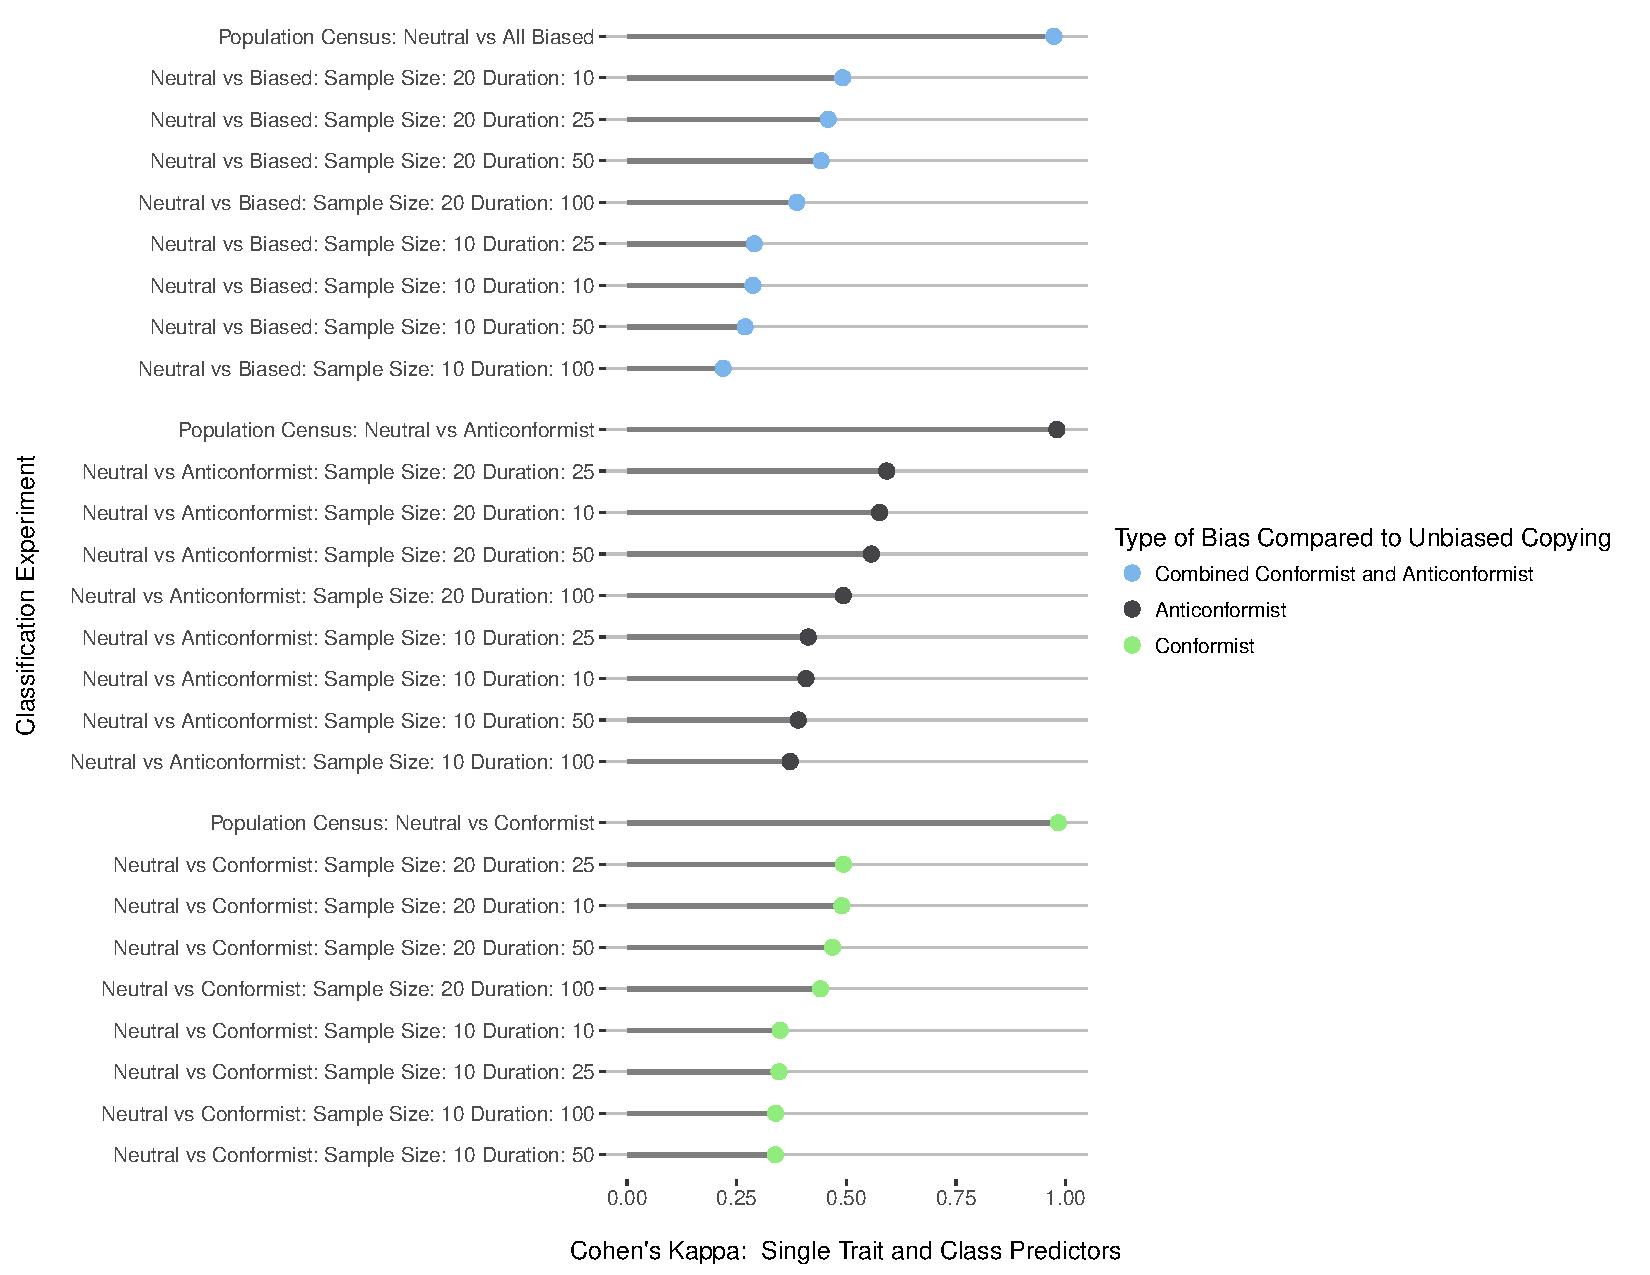
\includegraphics[scale=0.65]{graphics/ctmixtures/eq5-kappa-dotchart-full-predictors.pdf}
\caption{Cohen's kappa values for model comparisons, using a classifier trained on all predictors including per-locus and ``classes'' built from intersecting loci and then counting frequencies.  Top panel provides results for comparing a neutral, unbiased population and a balanced mixture of conformist and anti-conformists.  The middle panel provides results for unbiased compared to a population dominated by anti-conformists.  The bottom panel depicts results for unbiased compared toa population dominated by conformists.  Each panel presents results for the 9 data collection treatments analyzed.}
\label{ctmixtures:fig:kappa-full-predictors}
\end{figure}

\begin{figure}[p!]
\centering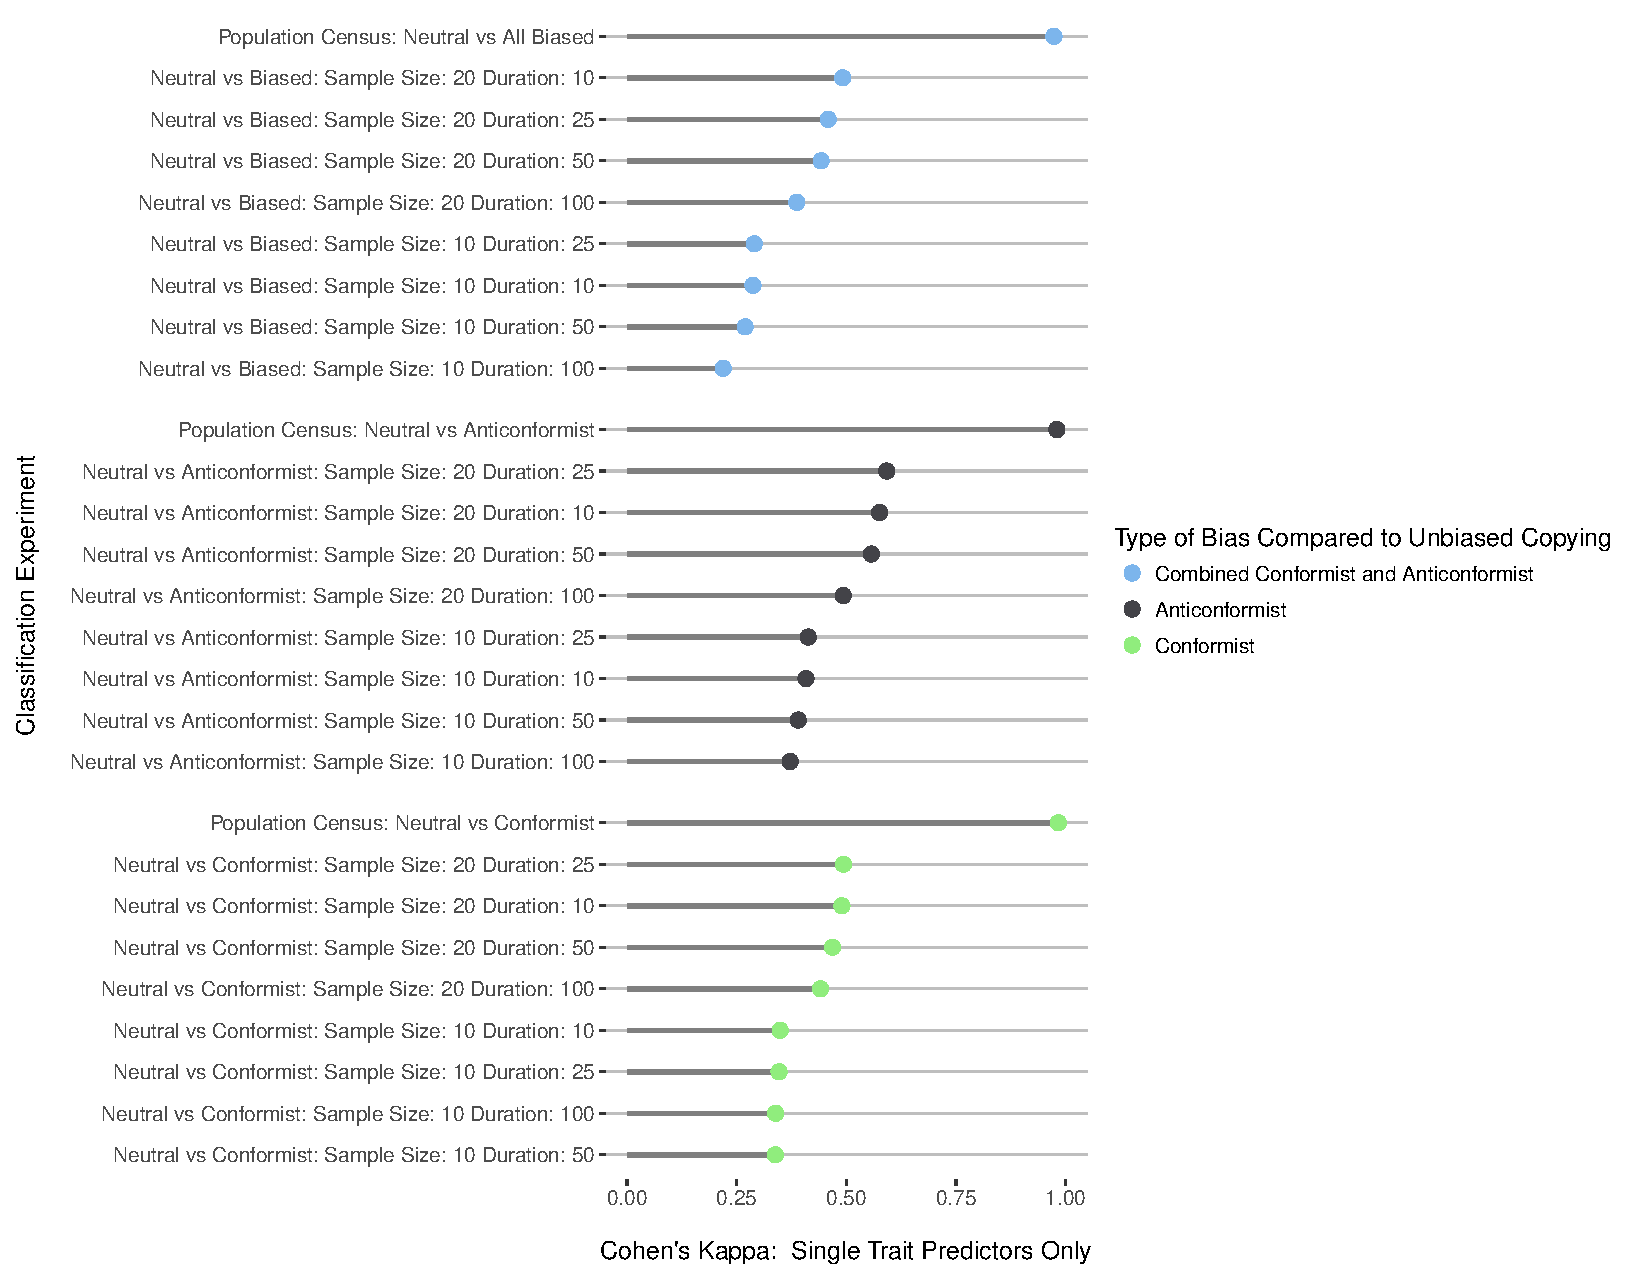
\includegraphics[scale=0.65]{graphics/ctmixtures/eq5-kappa-dotchart-perlocus-predictors.pdf}
\caption{Cohen's kappa values for model comparisons, using a classifier trained only on predictor variables derived from per-locus trait counts.  Top panel provides results for comparing a neutral, unbiased population and a balanced mixture of conformist and anti-conformists.  The middle panel provides results for unbiased compared to a population dominated by anti-conformists.  The bottom panel depicts results for unbiased compared toa population dominated by conformists.  Each panel presents results for the 9 data collection treatments analyzed.}
\label{ctmixtures:fig:kappa-perlocus-predictors}
\end{figure}

For each of the three comparisons, the Cohen's kappa scores were calculated two ways:  with all predictive variables (including the class variables measured on intersections of attributes from the 4 different loci), and for classifiers built only with per-locus variables (i.e., where we look only at what would be single attributes rather than more complex archaeological classes or culture-historical types.  

\subsection{Classification Error and Equifinality Results}

In this section I outline the results from the three model comparisons described above, across all 9 data collection treatments.  Figure \ref{ctmixtures:fig:kappa-full-predictors} depicts Cohen's kappa results for the classifier trained with all predictor variables, including those from per-locus trait counts, and those from intersecting all four loci into ``classes'' that mimic the way paradigmatic classifications are constructed to build archaeological types \citep{Dunnell1971}.  Figure \ref{ctmixtures:fig:kappa-perlocus-predictors} provides the Cohen's kappa results for the classifier trained only on predictor values derived from per-locus trait counts.  

What is strongly apparent, however, is population-level, coarse grained data \emph{can} reliably distinguish between a population of unbiased copiers and various mixtures of individuals with differing propensities for conformism and anti-conformism.  Using multiple variables in a classifier model creates sufficient discriminatory power that we can distinguish these models reliably, even in a balanced mixture with equal numbers of conformists and anti-conformists.  The effects do not, apparently, ``cancel out.''  

This ability to distinguish models, however, is only apparent where we can census the entire population (or, presumably take very large samples), and where there is no time averaging.  We should, in other words, expect to be able to identify pure and mixed models of social learning modes in situations where we can obtain synchronic samples, and capture enough of the population that we can accurately capture all of the variation present.  This is possible in experimental contexts, and in many contemporary data sets that represent data on whole populations.  That's good news for researchers seeking to use microevolutionary models to study social psychological phenomena related to social learning in contemporary contexts.

Even more strongly apparent, however, is that accuracy rapidly declines as sample fraction decreases and as time averaging increases.   As one might expect, larger samples offer more accurate predictions than smaller samples.  Within the larger, 20\% sample, when cross-tabulated class and per-locus predictors are included, accuracy is highest with the smallest amount of time averaging (10 generations), and decreases as time averaging increases.  When we remove cross-tabulated class predictors, and simply look at per-locus variables, this clean pattern is not apparent, and accuracy is not a function of time averaging duration.  Furthermore, for the smaller 10\% sample with all variables included, accuracy is not a function of time averaging duration.  In these cases, Cohen's kappa values are between 0.2 and 0.3, indicative of a very poor classification model with very little predictive power. 

While sample size is partially addressable in data collection, the degree to which archaeological deposits are aggregated over some window of time is often not alterable in research design.  There is equifinality here which we simply cannot avoid in most archaeological cases, which renders our ability to distinguish between realistic mixtures of social learning modes and unbiased copying unreliable at best, and impossible at worst.  

\subsection{Which Predictor Variables Help Discriminate Models?}

% \begin{table}[ht]
% \begin{tabular}{rc}
%   \hline
% Importance & Predictor Variable \\
%   \hline
% 100.00 & Cross-Tabulated Class Richness \\
%   50.71 & Slatkin Exact for Classes \\
%   29.50 & Shannon Entropy (Mean for Locus) \\
%   23.13 & Shannon Entropy for Classes \\
%   19.66 & IQV Diversity (Mean for Locus) \\
%   11.58 & Kandler-Shennan Trait Survival (Mean for Locus) \\
%   \hline
% \end{tabular}
% \caption{Relative importance of predictor variables for population census data, in the comparison between unbiased transmission and all biased models.  The most important variable is (by convention) scaled to 100, and the values indicate the ratio of variable importance to the variable which is most effective at classifying data points.  Only values greater than 10 are shown. The remainder of the predictor variables are 1/100th as effective as class richness or less.}
% \label{ctmixtures:tab:varimp-popcensus}
% \end{table}

Since there is some predictive power here, particularly using population census information, it is important to understand which variables were providing that discriminatory power.  
Gradient boosting algorithms allow measurement of how much each predictor variable contributes to a classification model.  The importance of a variable is assessed over the iterations of tree construction by estimating the relative improvement in training set misclassification error from adding the variable to the model.  The importance values are usually scaled such that the most important variable has a score of 100, and variables with smaller importance values are less important to classification power.  

In general the pattern is the same across comparisons, so I illustrate variable importance by examining the comparison between unbiased copiers, and the population composed of a balanced mixture of conformists and anti-conformists.  Table \ref{ctmixtures:tab:varimp-balbiased-census} gives the relative importance of predictor variables when the classifier includes classes created by intersecting the 4 loci with individual traits.

Most classificatory power in this comparison comes from the richness in the cross-tabulated classes.  In general, richness (whether class or per-locus) dominated all of the classifier models, which is not surprising given the central role of the amount of variation in mathematical treatments of the Wright-Fisher and Moran models \citep{Ewens2004}.  The second variable in importance in this comparison is the p-value for a Slatkin's ``exact'' test, which determines the probability that a given set of class frequencies come from the Ewens Sampling Distribution \citep{slatkin1994exact}.  The Shannon entropy, a measure of evenness in frequency (in this case averaged across loci) provides about half as much predictive power as richness. Interestingly the Kandler-Shennan survival time, averaged across the 4 loci, offers significant discriminatory power, suggesting that the method used here for simulating it along with time averaging is a fruitful avenue for additional research.  Beyond this, the predictors have increasingly little power, likely because we have multiple variants on evenness measures in the full list of summary statistics, and their results are collinear with other variables. 

\begin{table}[ht]
\begin{tabular}{rc}
  \hline
Importance & Predictor Variable \\
  \hline
100.00 & Cross-Tabulated Class Richness \\
  85.49 & Slatkin Exact for Classes \\
  47.12 & Shannon Entropy (Mean for Locus) \\
  24.12 & Kandler-Shennan Trait Survival (Mean for Locus) \\
  18.88 & IQV Diversity (Mean for Locus) \\
  10.85 & Shannon Entropy for Classes \\   
  \hline
\end{tabular}
\caption{Relative importance of predictor variables for population census data, in the comparison between unbiased transmission and a balanced mixture of pro- and anti-conformists.  The most important variable is (by convention) scaled to 100, and the values indicate the ratio of variable importance to the variable which is most effective at classifying data points. Only values greater than 10 are shown. The remainder of the predictor variables are 1/100th as effective as class richness or less.}
\label{ctmixtures:tab:varimp-balbiased-census}
\end{table}

\subsection{Time Averaging Makes Identification of Bias More Likely}

As shown in these results and previous studies \citep{Madsen2012,Porvcic2014,Premo2014}, the temporal aggregation we encounter in archaeological data is a significant barrier to discriminating between theoretical models of cultural transmission.  Equifinality increases as the amount of time averaging represented in a data set increases.  But this is not the whole story.  Time averaging, combined with sampling effects, do not simply make our classifiers worse in a random manner.  Instead, there is substantial bias in the pattern of classification (and thus model identification) errors.  

We can see this clearly by examining two confusion matrices from the comparison between unbiased and a balanced mixture of social learning biases.  Table \ref{ctmixtures:tab:confusion-matrix-census} shows the pattern of correct and incorrect predictions for the population census with no time averaging treatment.  In the confusion matrix, the rows depict the \emph{predicted} data generating model, and the columns provide the true data generating model.  Thus, in the row ``biased'', the first column are correct predictions that data points came from the mixture of biases model, while the second column are incorrect predictions that the data points arose from a model of bias, when the data points in fact arose from unbiased copying.

Even in the population census treatment, there is a slight tendency for prediction errors to be unbalanced.  It is more likely to misidentify a data point arising from unbiased copying as coming from a mixture of biased copiers than it is to make the opposite error.  In other words, we over-identify bias, even with complete data, by about 30%.  

Table \ref{ctmixtures:tab:confusion-matrix-sampledata} shows the pattern of errors for the same comparison, but with 20\% sample fraction and time averaging duration of 50 steps.  This is not the worst treatment for accuracy by far, but note that the pattern of errors has become significantly more asymmetric.  With this data collection treatment 2.7 times more likely that we will make an error favoring an identification as transmission bias than that we will misidentify bias as neutrality.  

\begin{table}[p!]
	
    \begin{tabular}{|c|c|c|}
      \hline
     & biased & neutral \\ 
      \hline
    biased & 14898 & 132 \\ 
      neutral & 102 & 4868 \\ 
       \hline
    \end{tabular}
    \caption{Confusion matrix for comparison of unbiased versus mixed bias models, for the data treatment with population census of trait frequencies and no time averaging.}
    \label{ctmixtures:tab:confusion-matrix-census}
\end{table}

\begin{table}[p!]

    %`Sample Size:  20  Duration:  50`
    \begin{tabular}{|c|c|c|}
      \hline
     & biased & neutral \\ 
      \hline
    biased & 13926 & 2724 \\ 
      neutral & 1074 & 2276 \\ 
       \hline
    \end{tabular}
    \caption{Confusion matrix for comparison of unbiased versus mixed bias models, for the data treatment with 20\% sampling fraction and 50 steps for time averaging duration.}
    \label{ctmixtures:tab:confusion-matrix-sampledata}
\end{table}

By looking at the ratio of the right column in each confusion matrix, across all data collection treatments, we can see how the magnitude of this asymmetric preference for identification of bias scales with sample size and duration of time averaging  (Table \ref{ctmixtures:tab:misclassification-neutral}).  The smaller our samples are from the original population, and the more temporal aggregation in our assemblages, the more likely we are to ``see'' biased cultural transmission, even with combinations of summary statistics and powerful classifier models.

\begin{table}[ht]

\begin{tabular}{|l|c|}
  \hline
Data Collection Treatment & \% of Unbiased Data Points Misclassified as Biased \\
  \hline
Population Census & 2.6 \\
  Per-Locus Population Census & 3.4 \\
  Sample Size:  20  Duration:  10 & 49.1 \\
  Sample Size:  20  Duration:  25 & 49.5 \\
  Per-Locus Sample Size:  20  Duration:  25 & 49.7 \\
  Per-Locus Sample Size:  20  Duration:  10 & 50.1 \\
  Per-Locus Sample Size:  20  Duration:  50 & 54.4 \\
  Sample Size:  20  Duration:  50 & 54.5 \\
  Sample Size:  20  Duration:  100 & 57.6 \\
  Per-Locus Sample Size:  20  Duration:  100 & 58.1 \\
  All Sample Sizes and TA Durations & 68.0 \\
  Per-Locus Sample Size:  10  Duration:  25 & 73.5 \\
  Sample Size:  10  Duration:  25 & 73.6 \\
  Sample Size:  10  Duration:  50 & 73.7 \\
  Per-Locus Sample Size:  10  Duration:  10 & 73.8 \\
  Per-Locus Sample Size:  10  Duration:  100 & 74.0 \\
  Per-Locus Sample Size:  10  Duration:  50 & 74.1 \\
  Sample Size:  10  Duration:  100 & 74.4 \\
  Sample Size:  10  Duration:  10 & 74.7 \\
   \hline
\end{tabular}

    \caption{Percentage of data points from the unbiased transmission model that are falsely identified as arising from a biased model.}
    \label{ctmixtures:tab:misclassification-neutral}
\end{table}


\section{Discussion}\label{ctmixtures:sec:conclusion}

The central aim in this study has been to examine whether realistic mixtures of social learning strategies present fundamental equifinalities that were impossible to distinguish using population level summary data.  The results demonstrate that mixtures of biased social learning strategies do not ``cancel out'' sufficiently to mask their statistical signatures---when you have enough data, synchronic observations, and use several summary statistics in combination.  

However, when time averaging is present, and especially with small sample sizes, our ability to discriminate between theoretical models essentially disappears.  Equifinality is omnipresent.  Even worse, the results indicate that our ability to distinguish between models does not degrade symmetrically.  In the presence of time averaging and with small samples, we are several times more likely to identify data points as arising from transmission bias than we are when we have synchronic and more complete data.  

Archaeologists engaged in the study of microevolutionary cultural transmission models should employ a healthy skepticism about the enterprise of fitting artifact class frequency data to models.  Even with diachronic methods such as trait survival \citep{Kandler2013}, multiple summary statistics, and powerful analytic methods, there is little evidence that we can distinguish these models with simulated data.  And that should give us great pause in thinking that our conclusions from analyzing archaeological samples are sound.  It is time to evaluate whether the application of microevolutionary models in archaeology is a fruitful enterprise, or whether our time is better spent deriving models which are robust in the face of time averaging---even if those models address larger scale questions instead of the social psychological questions involved in most dual inheritance theory.  

\textcolor{teal}{It is certainly true that evolutionary change is ultimately caused by individual variation and how that variation affects success.   In a sense, all evolutionary change is ``caused'' by that individual level variation; patterns and processes we observe at larger spatiotemporal scales and taxonomic levels are ``upper level effects'' of individual level variation \citep{walsh2019paradox}.  This does not make population, regional, and taxonomic level patterning in evolutionary history mere ``epiphenomena.''  Far from it.  The structure and history of populations and their environments provide the fitness landscapes which shape and sort variation among individuals.  Archaeology is uniquely placed not just to document variation at larger scales, but to study processes that are only operative at scales larger than individuals and single populations.}  

\textcolor{teal}{We do not have a complete catalog of evolutionary processes that can only be studied above the level of single populations, but there are numerous examples. Variation in traits which affect dispersal lead to phenotypic variation among populations depending upon their migration and dispersal characteristics, an effect that \citet{shine2011evolutionary} refer to as ``spatial sorting.''  We can and should expect such differences to be evidence at archaeological scales when we compare sedentary versus mobile communities in the archaeological record, for example.  Niche construction often occurs over evolutionary time \citep{Laland2000,Odling-Smee2003,Odling-Smee2007}, including all kinds of coevolutionary relationships such as domestication \citep{rindos1984origins}.  All of these processes require the time depth inherent in the archaeological record for proper study and explanation.  Large scale population structure---patterns in interaction between communities, is something we can document at mesoscopic and macroevolutionary scales, and is part of what we mean when we discuss ``social complexity.''  Building models for these kinds of processes requires tools for creating diachronic models and fitting them to coarse grained, time averaged data.  In the following chapters, I turn to several methods for creating such models and evaluating equifinality among them.  
}

